% =====================================================================
% PARTIE 4 : L'ETUDE ELECTRIQUE (etude electrique v2, texte integral)
\clearpage
\partieENO{L'étude électrique et l'énergie solaire}

La tour fonctionne sans prise de courant : tout vient du soleil. Cette partie reprend en entier l'étude électrique (version 2) de la tour, avec ses calculs, ses démonstrations, ses tableaux et son protocole de mesure. Elle répond, dans l'ordre, à quatre questions. Combien d'énergie la tour consomme-t-elle en une journée ? Le panneau de \qty{120}{Wc} en produit-il assez le pire mois ? Les batteries tiennent-elles la nuit et quelques jours sans soleil ? Quelles sections de câbles et quels fusibles faut-il pour que le montage reste sûr ? Je commence par présenter le système (5.1) et son schéma (5.2). Je calcule ensuite la consommation (5.3), puis je dimensionne le panneau (5.4) et les batteries (5.5). Je vérifie la tension réellement présente sur le réseau \qty{12}{V} (5.6), je choisis les câbles et les fusibles (5.7), puis je décris le protocole de mesure qui remplacera les hypothèses par des valeurs réelles (5.8). Je rassemble les hypothèses (5.9) et je termine par la synthèse (5.10).

\Needspace{8\baselineskip}\subsection{Présentation du système électrique}

La tour est alimentée uniquement par le soleil. L'énergie suit le chemin suivant. Le panneau TE1250 de \qty{120}{Wc} produit l'électricité. Le régulateur MPPT\ix{19} SLC-MT2024 (SLD Tech, \qty{20}{A}) l'adapte et charge les batteries, et des fusibles protègent chaque ligne. Les batteries de \qty{12}{V} (\qty{6}{Ah} et \qty{17}{Ah}, en parallèle) stockent pour la nuit. Un convertisseur UBEC\ix{17} transforme le \qty{12}{V} en \qty{5}{V} pour le Raspberry Pi et l'Arduino. La carte de puissance Adafruit 6318, à huit MOSFET\ix{15}, commande les pompes en \qty{12}{V}. Un capteur de courant INA260\ix{22} mesure la tension et le courant de la batterie. Le synoptique et la feuille d'alimentation et de puissance sont reproduits ci-dessous (ils figurent aussi en partie 8.1) ; la partie 5.2 explique comment les lire.

Les sept fonctions sont donc : produire (panneau), réguler et protéger (régulateur MPPT\ix{19} et fusibles), stocker (batteries), mesurer l'énergie (INA260\ix{22}), convertir (UBEC\ix{17}), décider (Raspberry Pi 3 B avec son dongle Wi-Fi) et lire et agir (Arduino Uno R3, carte MOSFET\ix{15}, pompes et capteurs : pH, EC, eTape\ix{23}, DS18B20\ix{24}, DHT20\ix{24}, lumière, accéléromètre LIS3DHTR, ADS1115\ix{16}).

Le schéma synoptique suivant regroupe ces éléments en blocs et montre comment ils sont reliés.

\begin{figure}[H]
\centering
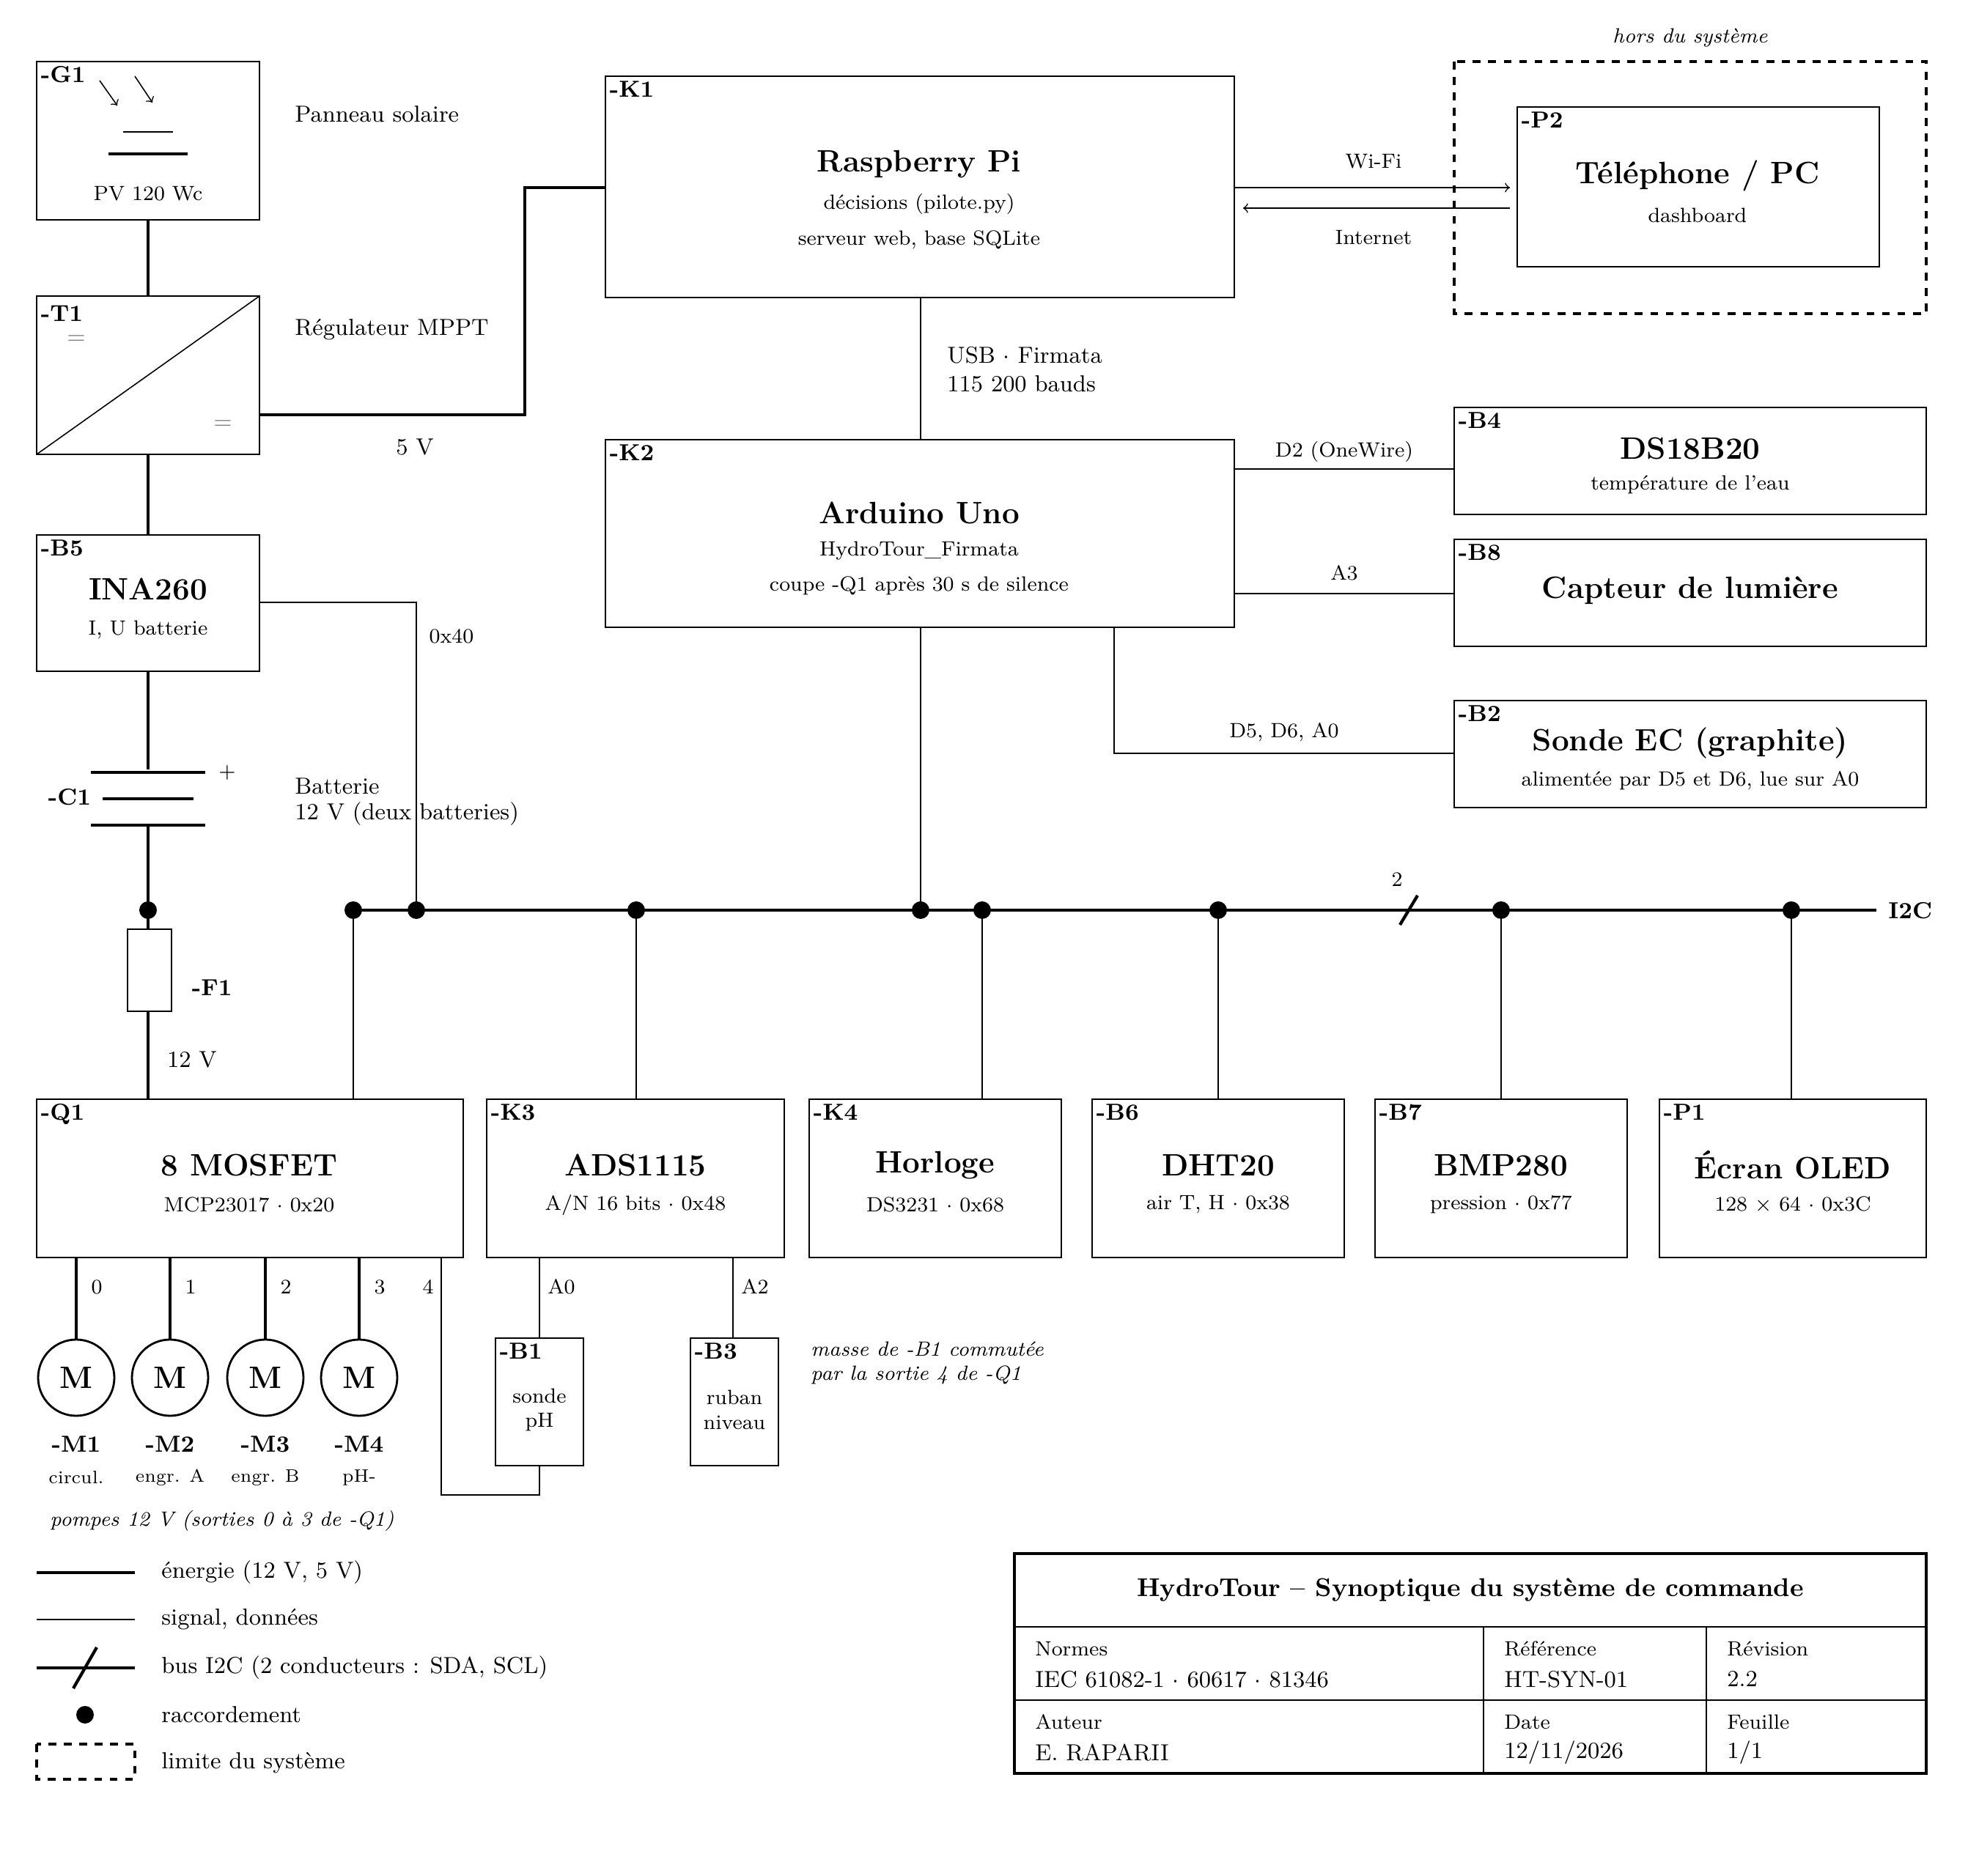
\includegraphics[width=\textwidth]{img/inf/f_synoptique.png}
\schemacap{synop}{Synoptique du système de commande (IEC 61082-1).}
\end{figure}

\schemapaysageC{eagle/schema_complet.pdf}{elcompl}{Schéma électrique complet de la tour (alimentation, commande, capteurs et sonde EC), sur une seule feuille.}


Le régulateur est un SLC-MT2024 : sa fiche (reproduite ci-dessous et dans l'Annexe 4) donne une tension d'entrée jusqu'à \qty{70}{V}, un courant de charge de \qty{20}{A}, une autoconsommation inférieure à \qty{15}{mA}, une charge en trois étages (absorption \qty{14,4}{V}, maintien \qty{13,8}{V}) et une coupure de charge à \qty{11,5}{V}. Ces réglages sont ceux d'une batterie au plomb. Mes batteries sont une Yuasa NP17-12I (\qty{17}{Ah}, plomb étanche) et une Steco YTX7A-BS (\qty{6}{Ah}, sans entretien, de type AGM). Le cahier des charges de départ parlait pourtant de batteries LiFePO4. Comme la technologie réelle se lit sur l'étiquette de chaque batterie, je calcule \textbf{les deux cas côte à côte} (LiFePO4 et plomb AGM) et je retiens le \textbf{plomb AGM} pour les conclusions de la tour, car c'est le cas défavorable et c'est celui des batteries que j'ai.

\schemapaysage[page=1]{SLC-MT2024.pdf}


\textbf{Conventions.} Les batteries sont des batteries de \qty{12}{V} nominal. Pour le LiFePO4, la tension moyenne en décharge vaut $U_B = \qty{12,8}{V}$ (4 éléments de \qty{3,2}{V}) ; pour le plomb AGM, $U_B = \qty{12,0}{V}$. Tous les courants côté \qty{12}{V} de la partie consommation sont calculés à \qty{12,8}{V} : à puissance égale, c'est le cas LiFePO4. Pour l'AGM, ces courants sont un peu plus forts, dans le rapport $12{,}8/12{,}0$, et les calculs correspondants sont donnés dans la partie 5.5.

\subsubsection*{Ce qui a changé depuis la version 1 de l'étude}

Cette version 2 reprend la structure, les données d'étiquette du panneau TE1250 et le rendement du convertisseur \qty{12}{V} vers \qty{5}{V} ($\eta = 0{,}83$) de la version 1. Les démonstrations sont réécrites et complétées. Le tableau résume les points qui changent.

\begin{table}[H]
\centering
\small
\begin{tabularx}{\textwidth}{|>{\raggedright\arraybackslash}p{2.6cm}|Y|Y|}
\hline
\textbf{Sujet} & \textbf{Version 1} & \textbf{Version 2} \\
\hline
Pompes & P1 à P5, dont une pompe d'appoint P5 et un bac de secours & Bac principal unique de \qty{152}{L}, appoint manuel. Pompes nommées par fonction : circulation, doseuses engrais A, engrais B, pH$-$ \\
\hline
Carte de puissance & Une sortie par pompe & Carte 6318 (8 MOSFET\ix{15}). Une sortie par pompe (circulation sur la sortie 0) \\
\hline
Capteurs & SHT31, BH1750, ADXL345, deux eTape\ix{23} & DHT, capteur de lumière analogique, LIS3DHTR (Sensor Kit), un seul eTape\ix{23}. pH sur l'entrée A1 de l'Arduino \\
\hline
Batteries & Plomb AGM supposé & LiFePO4 d'après le cahier des charges. Les deux cas sont calculés côte à côte (partie 5.5), la technologie réelle est à lire sur l'étiquette \\
\hline
Consommation & \qty{281}{Wh/j} & \qty{226,7}{Wh/j}. Écart surtout dû à l'électronique : \qty{91,8}{Wh/j} estimés composant par composant, contre \qty{149,8}{Wh/j} en version 1 (point d'essai du convertisseur à \qty{1}{A}). Pompe d'appoint retirée ; régulateur et MOSFET\ix{15} ajoutés. La mesure M2 tranchera \\
\hline
Production pire mois & \qty{336}{Wh/j} disponibles (avec $H = \qty{4,2}{kWh/m^2/j}$) & \qty{304,5}{Wh/j} (LiFePO4) ou \qty{272,4}{Wh/j} (AGM), avec $H = \qty{3,607}{kWh/m^2/j}$ en juin (Solargis) et des facteurs de pertes détaillés un par un \\
\hline
Fusibles & $F_{PV} = \qty{10}{A}$, $F_{B1} = \qty{5}{A}$, $F_{B2} = \qty{15}{A}$, $F_2 = \qty{7,5}{A}$ & $F_{PV}$, $F_{B1}$, $F_{B2}$ inchangés ; $F_2 = \qty{4}{A}$ (sans P5) ; nouveau $F_3 = \qty{2}{A}$ en entrée du convertisseur \qty{5}{V} \\
\hline
Calcul du panneau & Modèle à une diode, courbes du TE1250 à 25, 47, 50 et \qty{75}{\celsius} & Calcul direct sur le panneau entier, comparé aux mêmes courbes (écart inférieur à \qty{1}{\percent}) \\
\hline
Mesures & Absentes & Protocole complet, tableaux, fichiers modèles et script de traitement (partie 5.8) \\
\hline
\end{tabularx}
\caption{Ce qui change entre la version 1 et la version 2 de l'étude électrique.}
\end{table}

\begin{aretenir}
Sept fonctions : produire (panneau), réguler et protéger (MPPT\ix{19}, fusibles), stocker (batteries), mesurer l'énergie (INA260\ix{22}), convertir (UBEC\ix{17}), décider (Pi), lire et agir (Arduino, carte MOSFET\ix{15}, pompes, capteurs). Les deux technologies de batterie (LiFePO4 et plomb AGM) sont calculées ; l'AGM est retenu pour les conclusions.
\end{aretenir}

\Needspace{8\baselineskip}\subsection{Le schéma électrique}

Le schéma électrique complet est dessiné sur une seule feuille vectorielle (le zoom ne le floute pas), reproduite plus haut et en partie 8.1. Cette partie en donne la lecture et les règles de branchement.


\textbf{Lecture du schéma.} Les fils de puissance relient le panneau, le régulateur, les batteries, la carte MOSFET\ix{15} et le convertisseur. Les liaisons de données (bus I2C\ix{12}, signaux analogiques) sont dessinées à part. Chaque pompe se raccorde entre la borne $V+$ et la sortie MOSFET\ix{15} de son canal : la commutation se fait côté négatif, et la carte contient une diode de roue libre. La pompe de circulation est commandée par la sortie 0 de la carte (une sortie par pompe, partie 8.2). L'INA260\ix{22} est inséré entre la borne $BAT+$ du régulateur et le bus des batteries : il mesure le courant net (charge moins décharge) et la tension de la batterie. L'INA260\ix{22} est relié directement à l'Arduino (alimentation \qty{5}{V}, SDA\ix{13} et SCL\ix{14}) ; l'écran et les autres capteurs I2C\ix{12} sont sur un second bus de l'Arduino, qui leur fournit aussi le \qty{5}{V} et la masse ; le Raspberry Pi récupère la tension, le courant et le pourcentage de batterie auprès de l'Arduino. L'Arduino est alimenté en \qty{5}{V} et en données par l'USB du Raspberry Pi.



La notice du régulateur indique que c'est un contrôleur à positif commun : les bornes $PV+$, $BAT+$ et $LOAD+$ sont communes, et c'est le négatif qui est commuté. Les trois négatifs $PV-$, $BAT-$ et $LOAD-$ ne doivent donc jamais être reliés entre eux à l'extérieur. Chaque négatif va sur sa borne : le moins du panneau sur $PV-$, le moins des batteries sur $BAT-$, et la masse de la tour (carte MOSFET\ix{15}, UBEC\ix{17}, INA260\ix{22}) sur $LOAD-$.

\textbf{Ordre de branchement.} On branche d'abord les batteries, fusibles retirés jusqu'à la fin du câblage, puis le panneau. Le débranchement se fait dans l'ordre inverse. Cet ordre évite que le régulateur voie le panneau sans batterie, ce qui peut l'endommager.

\Needspace{8\baselineskip}\subsection{Le bilan de consommation}

\subsubsection*{Ce que je cherche et ce que je suppose}

Je cherche l'énergie $E_j$ consommée en une journée, en wattheures. Je la calcule composant par composant, en deux grands blocs : l'électronique alimentée en \qty{5}{V}, et ce qui est pris directement sur le \qty{12}{V} (pompes, pertes des MOSFET\ix{15}, autoconsommation du régulateur). Les courants de l'électronique sont des courants moyens en fonctionnement normal, estimés à partir des fiches techniques : ce sont des hypothèses, à vérifier par la mesure M2 (partie 5.8). La pompe de circulation de \qty{19}{W} tourne selon un planning, en heure de Tahiti : de 6 h à 18 h, \qty{15}{min} de marche puis \qty{15}{min} d'arrêt, soit 2 marches par heure pendant 12 h ; la nuit, \qty{15}{min} à 21 h, à 0 h et à 3 h.

\subsubsection*{L'électronique alimentée en 5 V}

Le Raspberry Pi, le dongle Wi-Fi, l'Arduino (par l'USB du Pi) et tous les capteurs sont alimentés en \qty{5}{V} par l'UBEC\ix{17}. Le tableau donne le courant moyen de chaque composant, sa puissance à \qty{5}{V} et son énergie sur 24 heures.

\begin{table}[H]
\centering
\small
\begin{tabularx}{\textwidth}{|>{\raggedright\arraybackslash}X|r|r|r|}
\hline
\textbf{Composant} & \textbf{$I$ moyen (mA)} & \textbf{$P$ à \qty{5}{V} (W)} & \textbf{$E$ sur \qty{24}{h} (Wh)} \\
\hline
Raspberry Pi 3 Model B (sans écran, charge faible) & 450 & 2,250 & 54,00 \\
\hline
Dongle Wi-Fi USB à antenne externe & 120 & 0,600 & 14,40 \\
\hline
Arduino Uno R3 & 50 & 0,250 & 6,00 \\
\hline
Base Grove (LED témoin) & 3 & 0,015 & 0,36 \\
\hline
Carte pH Gravity V2.0 & 5 & 0,025 & 0,60 \\
\hline
Sonde EC fabriquée (alimentée seulement à la lecture) & 0,2 & 0,001 & 0,02 \\
\hline
eTape\ix{23} \qty{30}{cm} et sa résistance de référence & 2 & 0,010 & 0,24 \\
\hline
ADS1115\ix{16} & 0,2 & 0,001 & 0,02 \\
\hline
DS18B20\ix{24} & 0,5 & 0,003 & 0,06 \\
\hline
Capteur d'humidité et de température de l'air & 0,3 & 0,002 & 0,04 \\
\hline
Capteur de lumière (analogique) & 0,5 & 0,003 & 0,06 \\
\hline
Accéléromètre LIS3DHTR & 0,02 & 0,000 & 0,00 \\
\hline
Module RTC (horloge) & 0,2 & 0,001 & 0,02 \\
\hline
INA260\ix{22} (partie logique) & 1,1 & 0,006 & 0,13 \\
\hline
Carte 6318 : MCP23017 et LED témoin & 2 & 0,010 & 0,24 \\
\hline
\textbf{Total côté \qty{5}{V}} & \textbf{635} & \textbf{3,175} & \textbf{76,20} \\
\hline
\end{tabularx}
\caption{Consommation moyenne de l'électronique alimentée en \qty{5}{V}.}
\end{table}

Le Raspberry Pi et le dongle Wi-Fi représentent à eux seuls \qty{90}{\percent} de la consommation de l'électronique : c'est là qu'une économie aurait un effet (désactiver le HDMI, les LED, le Bluetooth, le Wi-Fi interne si le dongle est utilisé).

\naturecalc{théorie (formule démontrée, valeurs de fiches techniques et hypothèses ; rien de mesuré)}
\begin{demonstration}[énergie consommée par un composant]
\resultat{E = P\,\Delta t}
Je note $P$ la puissance reçue par le composant, en watts, $U$ la tension à ses bornes, en volts, $I$ le courant qui le traverse, en ampères, $\Delta t$ la durée de fonctionnement, en heures, et $E$ l'énergie, en wattheures. La puissance instantanée reçue par un dipôle est le produit de la tension à ses bornes par le courant qui le traverse :
\begin{align*}
P &= U\, I
\end{align*}
L'énergie est l'intégrale de la puissance sur la durée $\Delta t$ :
\begin{align*}
E &= \int_{0}^{\Delta t} P(t)\,\mathrm{d}t
\end{align*}
Si $P$ est constante sur la durée de fonctionnement, elle sort de l'intégrale :
\begin{align*}
E &= P \int_{0}^{\Delta t} \mathrm{d}t\\
E &= P\,\Delta t
\end{align*}
Avec $P$ en watts et $\Delta t$ en heures, $E$ est en wattheures ($\qty{1}{Wh} = \qty{3600}{J}$). Pour un courant \emph{moyen} $\bar I$ sous tension constante, $\bar P = U \bar I$ donne la même énergie que le courant réel.
\end{demonstration}

\naturecalc{théorie (formule démontrée, valeurs de fiches techniques et hypothèses ; rien de mesuré)}
\begin{demonstration}[énergie de l'électronique alimentée en 5 V]
\resultat{E_5 = \qty{76,2}{Wh/j}}
Tous les composants sont en parallèle sur le \qty{5}{V} : leurs courants s'additionnent. Le courant total côté \qty{5}{V}, en ampères, vaut (somme de la colonne du tableau) :
\begin{align*}
I_5 &= \qty{0,635}{A}
\end{align*}
La puissance côté \qty{5}{V}, en watts, vaut :
\begin{align*}
P_5 &= U_5\, I_5\\
P_5 &= \qty{5,0}{V} \times \qty{0,635}{A}\\
P_5 &= \qty{3,175}{W}
\end{align*}
L'énergie sur une journée de \qty{24}{h} vaut :
\begin{align*}
E_5 &= P_5\,\Delta t\\
E_5 &= \qty{3,175}{W} \times \qty{24}{h}\\
E_5 &= \qty{76,2}{Wh/j}
\end{align*}
\end{demonstration}

\subsubsection*{Les pertes du convertisseur 12 V vers 5 V}

L'UBEC\ix{17} n'est pas parfait : il prend sur le \qty{12}{V} plus de puissance qu'il n'en rend sur le \qty{5}{V}, et la différence part en chaleur.

\naturecalc{théorie (formule démontrée, valeurs de fiches techniques et hypothèses ; rien de mesuré)}
\begin{demonstration}[puissance absorbée par un convertisseur]
\resultat{P_{entrée} = \dfrac{P_{sortie}}{\eta}}
Je note $\eta$ le rendement du convertisseur (sans unité), $P_{sortie}$ la puissance utile fournie, en watts, et $P_{entrée}$ la puissance absorbée, en watts. Le rendement est le rapport de la puissance utile fournie à la puissance absorbée :
\begin{align*}
\eta &= \frac{P_{sortie}}{P_{entrée}}
\end{align*}
J'isole la puissance d'entrée :
\begin{align*}
P_{entrée} &= \frac{P_{sortie}}{\eta}
\end{align*}
La puissance perdue (chaleur) est la différence, puis je factorise $P_{sortie}$ :
\begin{align*}
P_{pertes} &= P_{entrée} - P_{sortie}\\
P_{pertes} &= \frac{P_{sortie}}{\eta} - P_{sortie}\\
P_{pertes} &= P_{sortie}\left(\frac{1}{\eta} - 1\right)
\end{align*}
\end{demonstration}

\naturecalc{théorie (formule démontrée, valeurs de fiches techniques et hypothèses ; rien de mesuré)}
\begin{demonstration}[puissance prise sur le 12 V par l'électronique]
\resultat{E_{12,e} = \qty{91,8}{Wh/j}}
Je prends $\eta = 0{,}83$ (valeur de la version 1, à confirmer par la mesure M2) et $P_{sortie} = P_5 = \qty{3,175}{W}$. La puissance prise sur le \qty{12}{V} vaut :
\begin{align*}
P_{12,e} &= \frac{P_5}{\eta}\\
P_{12,e} &= \frac{\qty{3,175}{W}}{0{,}83}\\
P_{12,e} &\approx \qty{3,825}{W}
\end{align*}
La puissance perdue dans le convertisseur vaut :
\begin{align*}
P_{conv} &= P_5\left(\frac{1}{\eta} - 1\right)\\
P_{conv} &= \qty{3,175}{W} \times \left(\frac{1}{0{,}83} - 1\right)\\
P_{conv} &\approx \qty{0,650}{W}
\end{align*}
Le courant moyen pris sur la batterie par l'électronique, sous $U_B = \qty{12,8}{V}$, vaut :
\begin{align*}
I_{12,e} &= \frac{P_{12,e}}{U_B}\\
I_{12,e} &= \frac{\qty{3,825}{W}}{\qty{12,8}{V}}\\
I_{12,e} &\approx \qty{0,299}{A}
\end{align*}
L'énergie journalière prise sur le \qty{12}{V} vaut (dont $\qty{0,650}{W} \times \qty{24}{h} = \qty{15,6}{Wh}$ de pertes) :
\begin{align*}
E_{12,e} &= P_{12,e} \times \Delta t\\
E_{12,e} &= \qty{3,825}{W} \times \qty{24}{h}\\
E_{12,e} &\approx \qty{91,8}{Wh/j}
\end{align*}
\end{demonstration}

\subsubsection*{La pompe de circulation}

\naturecalc{théorie (formule démontrée, valeurs de fiches techniques et hypothèses ; rien de mesuré)}
\begin{demonstration}[durée de marche journalière et énergie de la pompe]
\resultat{t_c = \qty{6,75}{h/j} \quad\text{et}\quad E_c = \qty{128,25}{Wh/j}}
Je note $t_c$ la durée de marche par jour, en heures. De jour, il y a 12 heures et 2 marches de \qty{0,25}{h} par heure :
\begin{align*}
t_{jour} &= 12 \times 2 \times \qty{0,25}{h}\\
t_{jour} &= \qty{6,00}{h}
\end{align*}
De nuit (de 18 h à 6 h), il y a 3 marches de \qty{0,25}{h}, à 21 h, 0 h et 3 h :
\begin{align*}
t_{nuit} &= 3 \times \qty{0,25}{h}\\
t_{nuit} &= \qty{0,75}{h}
\end{align*}
\begin{align*}
t_c &= \qty{6,00}{h} + \qty{0,75}{h}\\
t_c &= \qty{6,75}{h/j}
\end{align*}
Avec la puissance $P_c = \qty{19}{W}$ de la pompe LPFIDI (donnée de la fiche), l'énergie d'après la démonstration précédente vaut :
\begin{align*}
E_c &= P_c\, t_c\\
E_c &= \qty{19}{W} \times \qty{6,75}{h/j}\\
E_c &= \qty{128,25}{Wh/j}
\end{align*}
Le courant de la pompe sous $U_B = \qty{12,8}{V}$ vaut :
\begin{align*}
I_c &= \frac{P_c}{U_B}\\
I_c &= \frac{\qty{19}{W}}{\qty{12,8}{V}}\\
I_c &\approx \qty{1,48}{A}
\end{align*}
\end{demonstration}

\subsubsection*{Les pertes dans les MOSFET de la carte 6318}

Chaque canal de la carte utilise un transistor MOSFET\ix{15} dont la résistance à l'état passant vaut $R_{DS(on)} = \qty{70}{m\ohm}$ (valeur de fiche du composant). La pompe de circulation est branchée sur un seul canal (sortie 0).

\naturecalc{théorie (formule démontrée, valeurs de fiches techniques et hypothèses ; rien de mesuré)}
\begin{demonstration}[pertes MOSFET\ix{15} de la circulation]
\resultat{E_{MOS} \approx \qty{1,04}{Wh/j}}
Je note $I$ le courant de la pompe, en ampères, et $U_{DS}$ la tension aux bornes du MOSFET\ix{15}, en volts. Un MOSFET\ix{15} saturé se comporte comme une résistance $R_{DS(on)}$. La loi d'Ohm donne $U_{DS} = R_{DS(on)}\, I$, donc la puissance dissipée, en watts, vaut :
\begin{align*}
P_1 &= U_{DS}\, I\\
P_1 &= R_{DS(on)}\, I^2
\end{align*}
Avec $I = I_c = \qty{1,48}{A}$ :
\begin{align*}
P_1 &= \qty{0,070}{\ohm} \times (\qty{1,48}{A})^2\\
P_1 &\approx \qty{0,154}{W}
\end{align*}
L'énergie perdue par jour, pendant $t_c = \qty{6,75}{h}$, vaut :
\begin{align*}
E_{MOS} &= P_1\, t_c\\
E_{MOS} &= \qty{0,154}{W} \times \qty{6,75}{h}\\
E_{MOS} &\approx \qty{1,04}{Wh/j}
\end{align*}
\end{demonstration}

\subsubsection*{Les pompes doseuses}

Les trois pompes péristaltiques\ix{8} (engrais A, engrais B, pH$-$) absorbent environ $I_d = \qty{0,30}{A}$ sous \qty{12}{V} et débitent environ $Q = \qty{80}{mL/min}$ en charge (hypothèse, à mesurer : mesure M5). Leur puissance sous $U_B = \qty{12,8}{V}$ vaut :
\begin{align*}
P_d &= U_B\, I_d\\
P_d &= \qty{12,8}{V} \times \qty{0,30}{A}\\
P_d &= \qty{3,84}{W}
\end{align*}

Pour estimer le volume d'engrais dosé par jour, je pars du fait que les laitues prélèvent les sels minéraux, donc que l'EC baisse. Je suppose une baisse de $\Delta EC = \qty{0,05}{mS/cm}$ par jour dans le bac de $V_{bac} = \qty{152}{L}$, et une solution mère telle qu'ajouter \qty{1}{mL} de A et \qty{1}{mL} de B par litre d'eau augmente l'EC de $s = \qty{0,56}{mS/cm}$ (hypothèses à confirmer par l'étude hydraulique et chimique).

\naturecalc{théorie (formule démontrée, valeurs de fiches techniques et hypothèses ; rien de mesuré)}
\begin{demonstration}[volume de solution mère pour corriger l'EC]
\resultat{V_A = \dfrac{\Delta EC\; V_{bac}}{s} \approx \qty{13,6}{mL/j}}
Je note $d$ la dose de solution mère par litre de bac, en mL/L, $V_A$ le volume ajouté, en mL, et $Q$ le débit de la pompe, en mL/min. En solution diluée, l'EC est proportionnelle à la concentration en sels, donc à la dose :
\begin{align*}
\Delta EC &= s\, d
\end{align*}
La dose est le volume ajouté divisé par le volume du bac :
\begin{align*}
d &= \frac{V_A}{V_{bac}}
\end{align*}
Je remplace et j'isole $V_A$ :
\begin{align*}
\Delta EC &= s\,\frac{V_A}{V_{bac}}\\
V_A &= \frac{\Delta EC\; V_{bac}}{s}
\end{align*}
La durée de fonctionnement d'une pompe de débit $Q$ est le volume divisé par le débit :
\begin{align*}
t &= \frac{V}{Q}
\end{align*}
Application, avec $s = \qty{0,56}{(mS/cm)/(mL/L)}$ :
\begin{align*}
V_A &= \frac{\qty{0,05}{mS/cm} \times \qty{152}{L}}{\qty{0,56}{(mS/cm)/(mL/L)}}\\
V_A &\approx \qty{13,6}{mL/j}
\end{align*}
Le même volume d'engrais B est dosé : $V_B = \qty{13,6}{mL/j}$. Pour le pH$-$, je suppose $V_{pH} = \qty{6}{mL/j}$. Les durées de marche valent :
\begin{align*}
t_A &= \frac{\qty{13,6}{mL}}{\qty{80}{mL/min}} = \qty{0,170}{min} = \qty{10,2}{s}\\
t_B &= \qty{10,2}{s}\\
t_{pH} &= \frac{\qty{6}{mL}}{\qty{80}{mL/min}} = \qty{0,075}{min} = \qty{4,5}{s}
\end{align*}
L'énergie estimée vaut :
\begin{align*}
E_{d,est} &= \qty{3,84}{W} \times \frac{(10{,}2 + 10{,}2 + 4{,}5)\,\unit{s}}{\qty{3600}{s/h}}\\
E_{d,est} &\approx \qty{0,027}{Wh/j}
\end{align*}
Valeur retenue (majorant) : le programme limite chaque commande à \qty{30}{s}. Je suppose au plus 10 commandes de \qty{30}{s} par pompe et par jour (cas d'un dérèglement) :
\begin{align*}
E_d &= 3 \times 10 \times \qty{30}{s} \times \frac{\qty{3,84}{W}}{\qty{3600}{s/h}}\\
E_d &= \qty{0,96}{Wh/j}
\end{align*}
\end{demonstration}

\subsubsection*{L'autoconsommation du régulateur}

\naturecalc{théorie (formule démontrée, valeurs de fiches techniques et hypothèses ; rien de mesuré)}
\begin{demonstration}[autoconsommation du régulateur MPPT\ix{19}]
\resultat{E_{MPPT\ix{19}} \approx \qty{4,61}{Wh/j}}
Le régulateur consomme un courant propre $I_{MPPT} = \qty{15}{mA}$ (valeur de la fiche), jour et nuit, sous $U_B = \qty{12,8}{V}$ :
\begin{align*}
P_{MPPT} &= U_B\, I_{MPPT}\\
P_{MPPT} &= \qty{12,8}{V} \times \qty{0,015}{A}\\
P_{MPPT} &= \qty{0,192}{W}
\end{align*}
\begin{align*}
E_{MPPT} &= P_{MPPT} \times \qty{24}{h}\\
E_{MPPT} &= \qty{0,192}{W} \times \qty{24}{h}\\
E_{MPPT} &\approx \qty{4,61}{Wh/j}
\end{align*}
\end{demonstration}

\subsubsection*{L'énergie journalière totale}

Le tableau suivant additionne les consommations de chaque élément pour donner le bilan journalier de la tour.

\begin{table}[H]
\centering
\small
\begin{tabular}{|l|r|r|r|}
\hline
\textbf{Poste} & \textbf{$P$ (W)} & \textbf{Durée (h/j)} & \textbf{$E$ (Wh/j)} \\
\hline
Électronique \qty{5}{V} (vue du \qty{12}{V}, pertes UBEC\ix{17} comprises) & 3,825 & 24 & 91,81 \\
\hline
\quad dont pertes du convertisseur & 0,650 & 24 & 15,61 \\
\hline
Pompe de circulation & 19,0 & 6,75 & 128,25 \\
\hline
Pertes MOSFET\ix{15} circulation (un canal) & 0,154 & 6,75 & 1,04 \\
\hline
Pompes doseuses (majorant) & 3,84 & 0,25 & 0,96 \\
\hline
Autoconsommation du MPPT\ix{19} & 0,192 & 24 & 4,61 \\
\hline
\textbf{Total} & & & \textbf{226,7} \\
\hline
\end{tabular}
\caption{Bilan de consommation journalière de la tour.}
\end{table}

\naturecalc{théorie (formule démontrée, valeurs de fiches techniques et hypothèses ; rien de mesuré)}
\begin{demonstration}[énergie journalière totale]
\resultat{E_j \approx \qty{226,7}{Wh/j}}
Je somme tous les postes (ceux du tableau, hors la ligne « dont pertes », déjà comptée dans l'électronique) :
\begin{align*}
E_j &= E_{12,e} + E_c + E_{MOS} + E_d + E_{MPPT}\\
E_j &= \qty{91,81}{Wh/j} + \qty{128,25}{Wh/j} + \qty{1,04}{Wh/j} + \qty{0,96}{Wh/j} + \qty{4,61}{Wh/j}\\
E_j &= \qty{226,67}{Wh/j}\\
E_j &\approx \qty{226,7}{Wh/j}
\end{align*}
La pompe de circulation pèse $\qty{128,25}{Wh/j}/\qty{226,7}{Wh/j} \approx 57\,\%$ du total, l'électronique $\qty{91,8}{Wh/j}/\qty{226,7}{Wh/j} \approx 40\,\%$.
\end{demonstration}

La figure suivante montre la part de chaque élément dans la consommation journalière de \qty{227}{Wh/j}.

\begin{figure}[H]
\centering
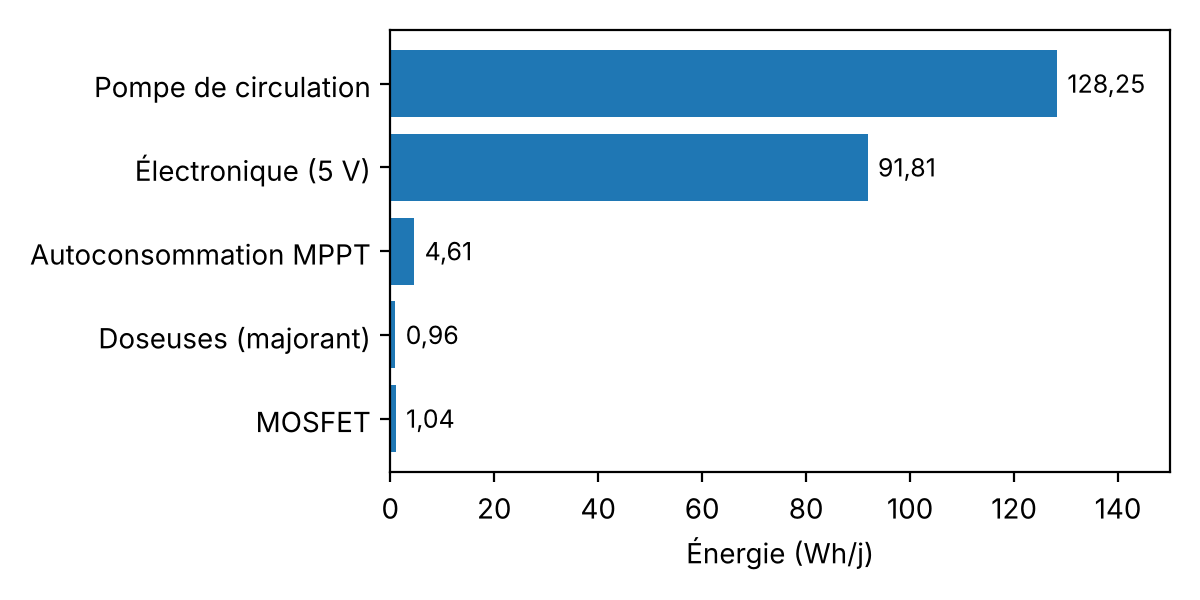
\includegraphics[width=0.78\textwidth]{img/conso.png}
\caption{Répartition de la consommation journalière : \qty{227}{Wh/j} au total.}
\end{figure}

\begin{aretenir}
Besoin journalier : $E_j = \qty{226,7}{Wh/j}$ (version 1 : \qty{281}{Wh/j}). Circulation \qty{128,25}{Wh} (57\,\%), électronique \qty{91,8}{Wh} (40\,\%) dont \qty{15,6}{Wh} de pertes du convertisseur, doseuses moins de \qty{1}{Wh}. Courant de repos sur le \qty{12}{V} : environ \qty{0,31}{A} ; courant de la pompe de circulation : \qty{1,48}{A}. Les pertes du MOSFET\ix{15} (un seul canal) valent \qty{0,154}{W}, soit \qty{1,04}{Wh/j}. La seule économie sérieuse possible est de réduire le temps de marche de la pompe ou la consommation du Raspberry Pi.
\end{aretenir}
